%%%%%%%%%%%%%%%%%%%%%%%%%%%%%%%%%%%%%%%%!TEX program = pdflatex

\documentclass[tikz]{standalone}

\usepackage{mathpazo,graphicx}

\begin{document}

\begin{tikzpicture}
    % 引入图片
    \node[anchor=south west,inner sep=0] (image) at (0,0) {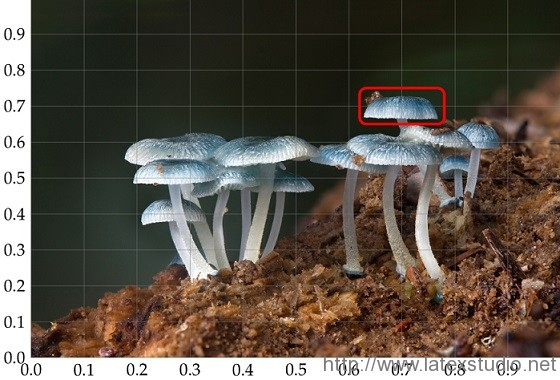
\includegraphics[width=0.9\textwidth]{test}};

    \begin{scope}[x={(image.south east)},y={(image.north west)}]
        % 建立相对坐标系
        \draw[help lines,xstep=.1,ystep=.1] (0,0) grid (1,1);
        \foreach \x in {0,1,...,9} { \node [anchor=north] at (\x/10,0) {0.\x}; }
        \foreach \y in {0,1,...,9} { \node [anchor=east] at (0,\y/10) {0.\y}; }
        % 作图命令
        \draw[red, ultra thick, rounded corners] (0.62,0.65) rectangle (0.78,0.75);
    \end{scope}
\end{tikzpicture}

\end{document}

